\section{Thermal Diffusivity Sensitivity Validation}\label{sec:diffusivity}
The thermal diffusivity, $\alpha_{th}$ of geologic repository host media 
describes the tendency of thermal energy to diffuse through, and therefore be 
deposited, in the medium.

\subsection{LLNL Model Results}

In the creation of the \gls{STC} database, the thermal diffusivity was varied 
across a broad domain for each isotope, $i$, package spacing, $s$, limiting 
radius $r_{calc}$, and thermal conductivity $K_{th}$, considered.  By 
varying the thermal diffusivity of the repository model from $0.1-3\times 
10^{-6} [m^2\cdot s^{-1}]$, this sensitivity analysis succeeds in capturing the domain of 
thermal diffusivities witnessed in high thermal diffusivity salt deposits as 
well as low thermal diffusivity clays.

\begin{figure}[htbp!]
\begin{center}
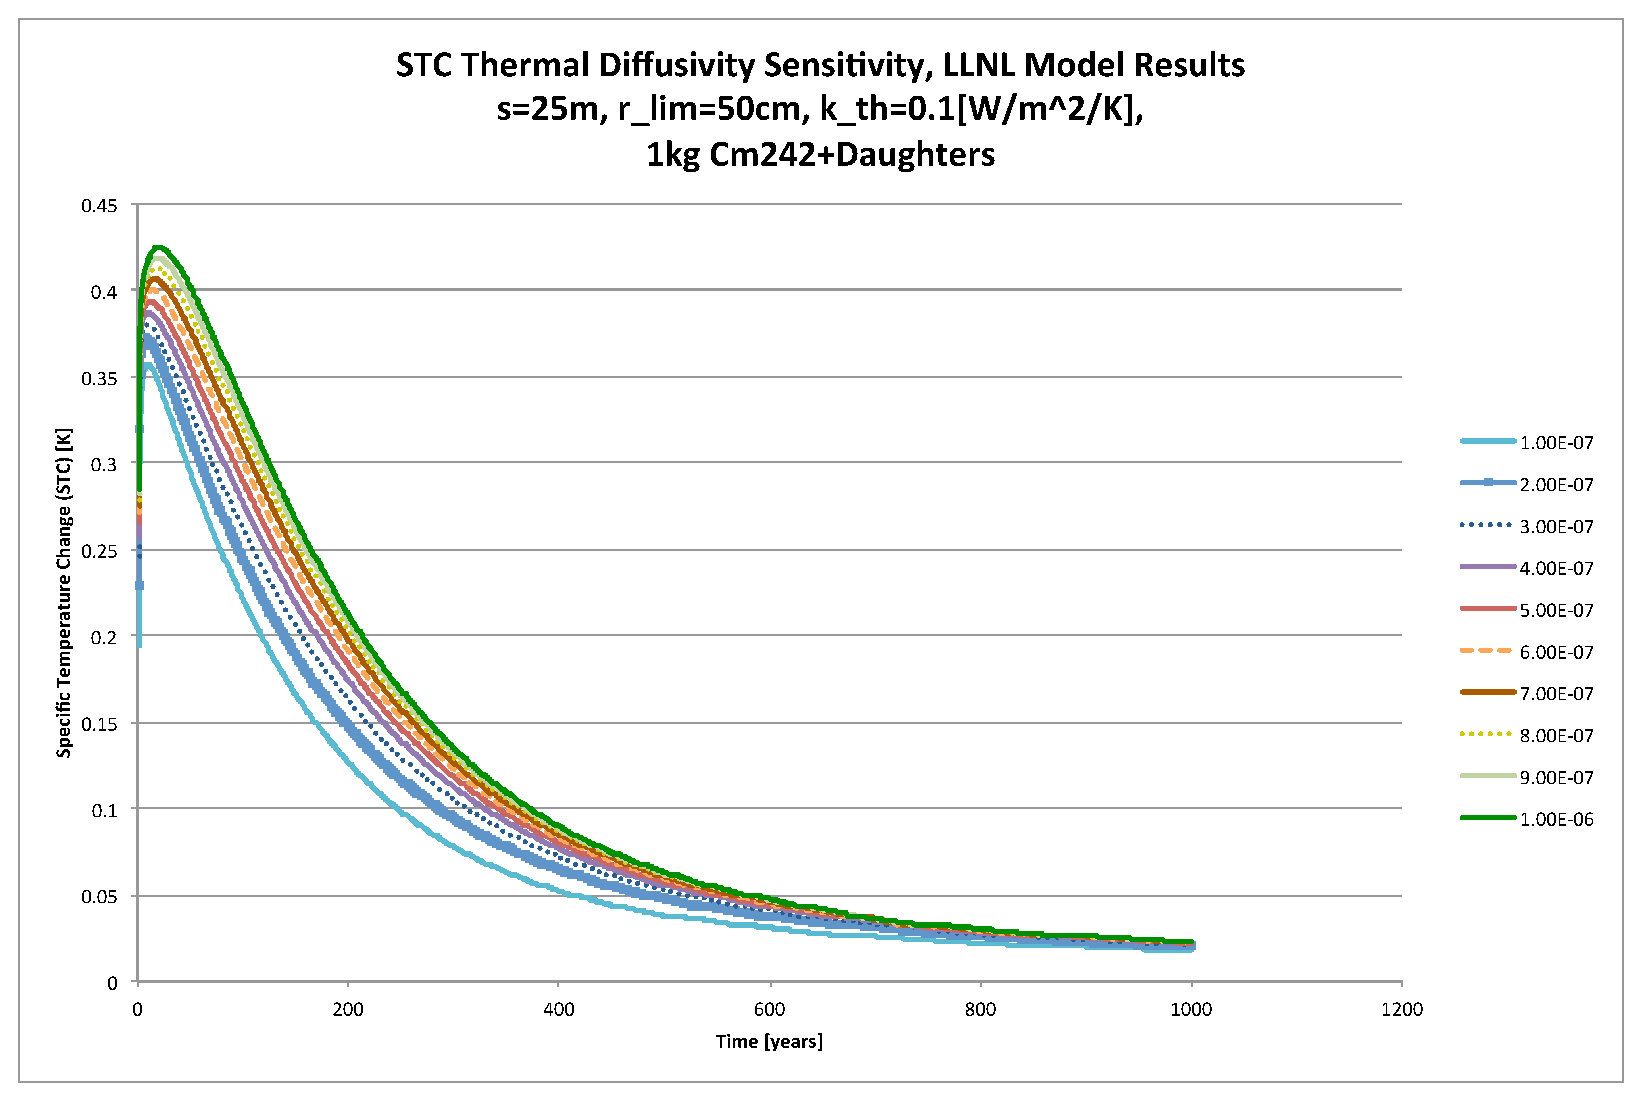
\includegraphics[width=0.7\textwidth]{./chapters/demonstration/diffusivity/Cm242alpha_kth_low.eps}
\end{center}
\caption[$K_{th}$ Sensitivity to $\alpha_{th}$ for $k_{th}$]{Increased thermal diffusivity decreases thermal energy deposition 
(here represented by \gls{STC}) in the near field (here $r_{calc} = 0.5m$).}
\label{fig:Cm242alpha_kth_low}
\end{figure}


Figure \ref{fig:Cm242alpha_kth_low} shows the trend, visible for all isotopes, 
that increased thermal diffusivity of a medium decreases thermal energy 
deposition in the near field. This indicates, then that thermal diffusivity is 
an important parameter for repository geolgic medium selection. The effect is 
accentuated by high thermal conductivities, as seen in 
Figure \ref{fig:Cm242alpha_kth_high}

\begin{figure}[htbp!]
\begin{center}
%\includegraphics[width=0.7\textwidth]{./chapters/demonstration/diffusivity/Cm242alpha_kth_high.eps}
\end{center}
\caption[$K_{th}$ Sensitivity for High $\alpha_{th}$]{Increased thermal diffusivity decreases thermal energy deposition 
(here represented by \gls{STC}) in the near field (here $r_{calc} = 0.5m$).}
\label{fig:Cm242alpha_kth_high}
\end{figure}


\subsection{Cyder Results}

In a similar analysis, the thermal diffusivity was compared both with the 
spacing between waste packages and the limiting radius. 

Figures \ref{fig:kr} and \ref{fig:ks} validate the trend noted above that 
increased thermal diffusivity of a medium decreases thermal energy deposition 
in the near field.  Additionally, analysis with the \Cyder STC database 
demonstrates the way in which the importance of $K_{th}$ remains constant, but 
the importance of the limiting radius decreases with increasing $\alpha_{th}$.

\begin{figure}[htbp!]
\begin{center}
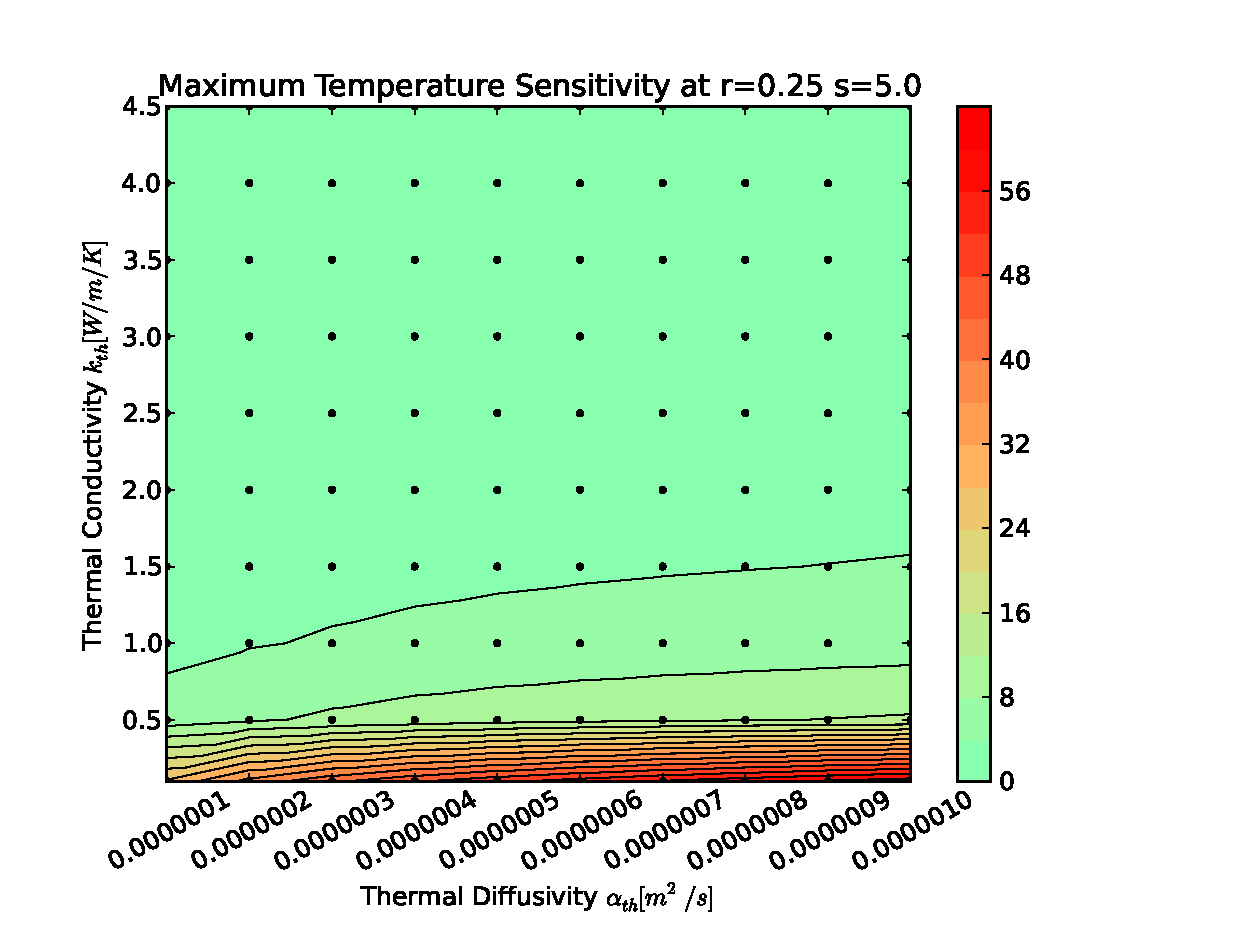
\includegraphics[width=0.7\textwidth]{./chapters/demonstration/diffusivity/ak.eps}
\end{center}
\caption[$\alpha_{th}$ vs. $K_{th}$ Sensitivity in Cyder]{Cyder results agree 
with those of the LLNL model, in which increased thermal diffusivity results in 
decreased thermal depsoition in the near field. The above example thermal 
profile results from 10kg of $^{234}Cm$} 
\label{fig:ar}
\end{figure}


\begin{figure}[htbp!]
\begin{center}
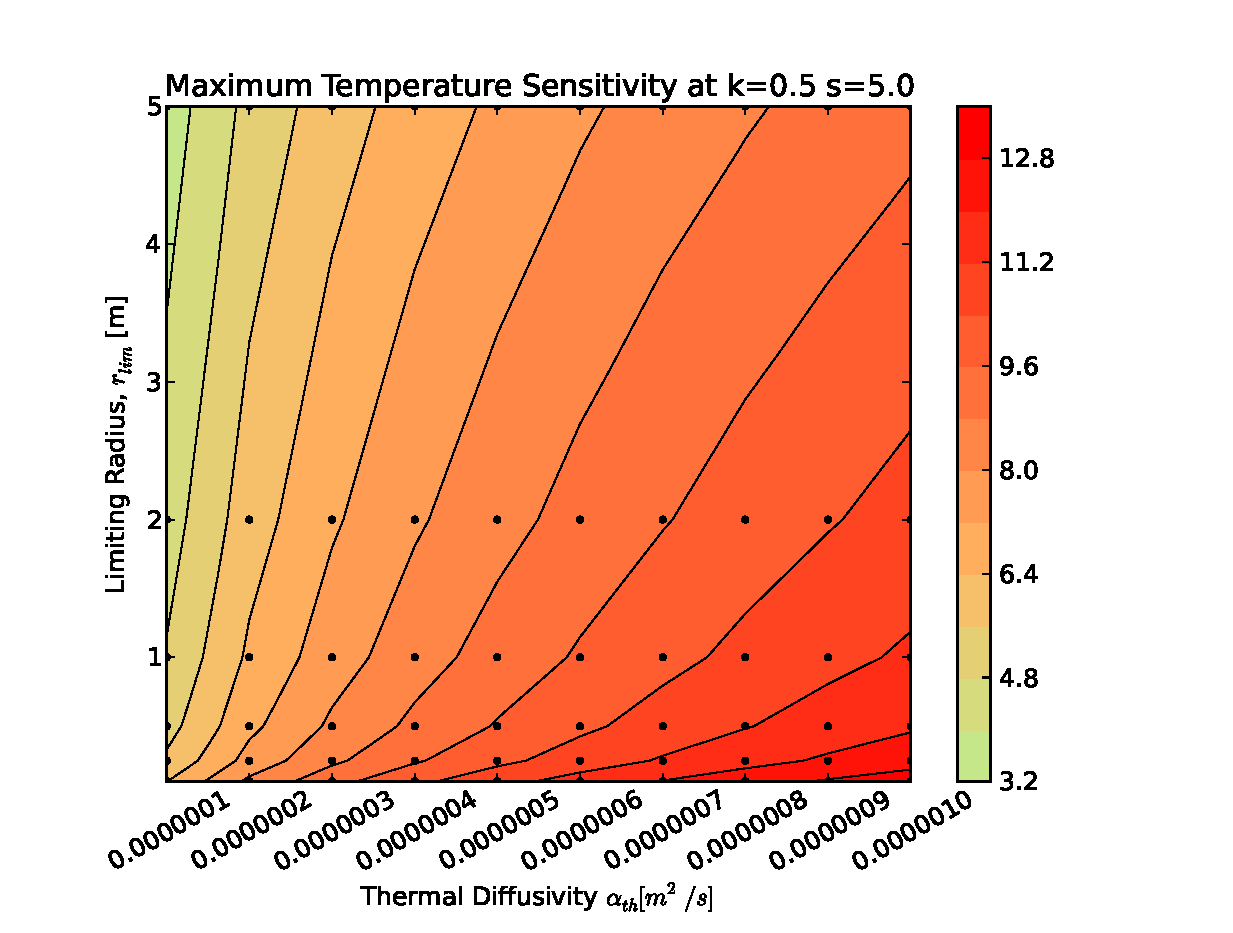
\includegraphics[width=0.7\textwidth]{./chapters/demonstration/diffusivity/ar.eps}
\end{center}
\caption[$\alpha_{th}$ vs. $r_{lim}$ Sensitivity in Cyder]
{Cyder results agree with 
those of the LLNL model. The importance of the limiting radius decreases with 
increased $K_{th}$. The above example thermal profile results from 10kg of 
$^{234}Cm$}
\label{fig:ak}
\end{figure}
